\documentclass[a4paper, 12pt, AutoFakeBold]{report}
%%% ========== Settings ==========
\usepackage[total={7in,10in}]{geometry}
% ---------- Chinese ----------
\usepackage{xeCJK}
\usepackage{indentfirst}
\XeTeXlinebreaklocale "zh"
\XeTeXlinebreakskip = 0pt plus 1pt
\setlength{\parindent}{2em}

% ---------- Fonts ----------
\usepackage{fontspec}
\setmainfont{Times New Roman}
\renewcommand{\familydefault}{\rmdefault}
\setCJKmainfont{標楷體}

% ---------- Formating ----------
\usepackage{listings}       % Script listing package
\usepackage{graphicx}       % Scalebox package
\usepackage{multicol}
\usepackage{caption}
\usepackage{subcaption}

% ---------- Math ----------
\usepackage{amsmath}        % Math matrix package
\usepackage{amssymb}        % Math symbols
\usepackage{resizegather}   % Math gather resizing

% ---------- Figure ----------
\usepackage{float}          % For figure [H] parameter place the graph
\usepackage{wrapfig}        % Wrap Figure or table package

% ---------- Table ----------
\usepackage{multirow}
\usepackage{makecell}
\usepackage{array}          % Tabular "m" parameter

% ---------- Other ----------
\usepackage{pdfpages}
\usepackage{hyperref}
\usepackage[toc]{appendix}

% ---------- Commands ----------
\newcommand{\figref}[1]{Fig.\ref{#1}}
\newcommand{\tabref}[1]{Tab.\ref{#1}}
\newcommand{\chref}[1]{Ch.\ref{#1}}
\hypersetup{hidelinks}

%%% ========== Document ==========
\begin{document}
    \tableofcontents
   %%% ==================== Electronic components ====================
    \chapter{Electronic Components}
    \section{Resistor}
    Under normal circumstances, in order to prevent the LED from being damaged due to an excessively high voltage applied to the LED, a control resistor is used to limit the flow of current to make the circuit operate smoothly.
    \begin{figure}[H]
        \centering
        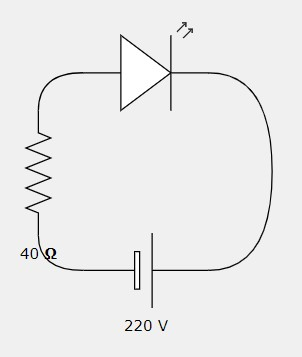
\includegraphics[scale=.7]{figs/Fig1-1.jpg}
        \caption{}
        \label{fig:1.1}
    \end{figure}

    \subsection{Variable resistor(Potentiometer)}
    Different from general resistors, it has three terminals. When in use, by changing the resistance value between the sliding end and the two fixed ends, different voltage division ratios are formed, so as to change the potential of the sliding point.

    \section{Operational Amplifier}
    Basically, an operational amplifier has two inputs (inverting and non-inverting) and one output.And the operational amplifier will generate two different outputs according to whether the voltage passed in by Vp is greater than Vn like \textbf{Figure 2.7}.
    \begin{figure}[H]
        \centering
        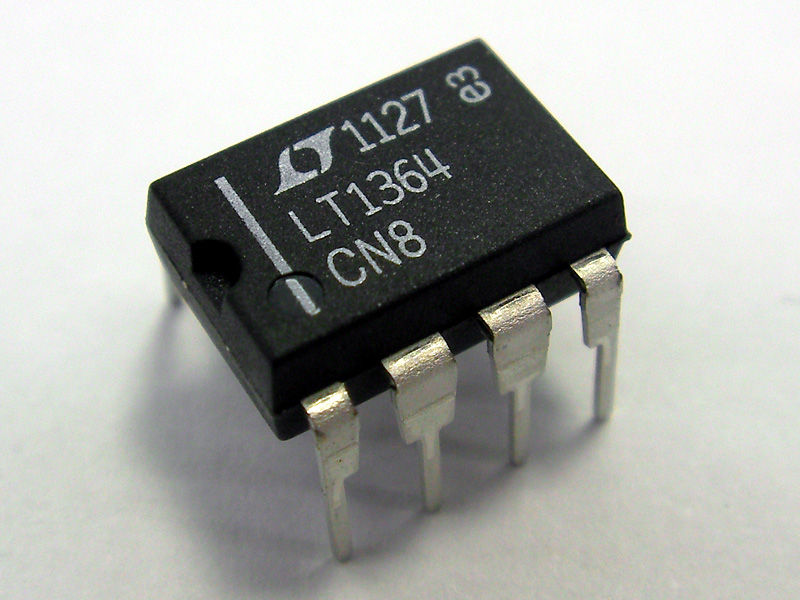
\includegraphics[scale=.3]{figs/Fig1-2.jpg}
        \caption{}
        \label{fig:1.2}
    \end{figure}

    \section{Power supply}
    In order to supply the electronic power, we at least use two 9V batteries in this project because we need both positive (+) and negative (-) voltages like \figref{fig:1.3}.
    \begin{figure}[H]
        \centering
        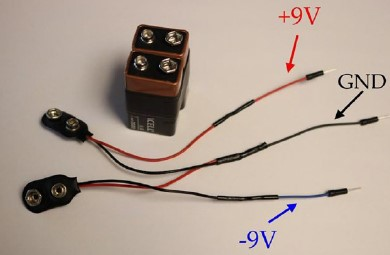
\includegraphics[scale=1]{figs/Fig1-3.jpg}
        \caption{}
        \label{fig:1.3}
    \end{figure}
    \noindent Need to pay attention when implementing
    \begin{itemize}
        \item how the battery clips are wired
        \item Ensuring the supply voltages are stable even under varying load conditions, you can use a +5V regulator and a -5V regulator.
    \end{itemize}

    \subsection{Voltage regulator}
    The purpose of a voltage regulator is to provide a stable voltage that does not change under different load conditions, and when wiring up these regulators, remember their "pin out." which the function of each pin is different, as shown in \figref{fig:1.3.1}.
    \begin{figure}[H]
        \centering
        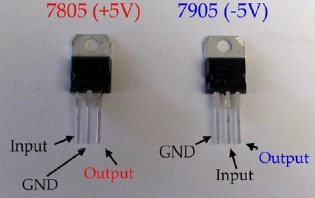
\includegraphics[scale=1]{figs/Fig1-3-1.jpg}
        \caption{}
        \label{fig:1.3.1}
    \end{figure}

    \section{LED}
    LEDs are often used to identify whether current is looping in a circuit, with shorter legs of cathode and longer legs of anode. \textbf{In circuit diagrams, LEDs are sometimes represented as resistors}
    \begin{figure}[H]
        \centering
        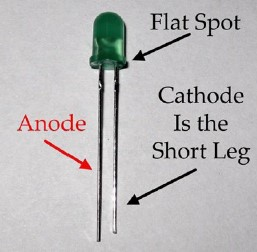
\includegraphics[scale=1]{figs/Fig1-4.jpg}
        \caption{}
        \label{fig:1.4}
    \end{figure}

    \section{SPDT switch}
    In order to have two dissimilar outputs to the network, a SPDT could switch two different paths of circuits by using a switch which as shown \figref{fig:1.5}, and can be done manually or included through the electromagnetic coil.
    \begin{figure}[H]
        \centering
        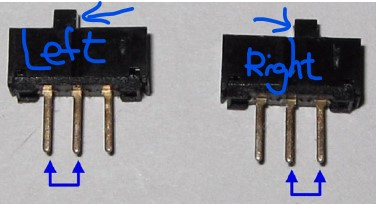
\includegraphics[scale=1]{figs/Fig1-5.jpg}
        \caption{}
        \label{fig:1.5}
    \end{figure}

   %%% ==================== Basic circuit ====================
    \chapter{Basic Circuit}
    \section{Voltages Summing}
    \label{ch:Voltage_sum}
    The \figref{fig:Summation_circuit} is the summation circuit. By KCL(Kirchhoff's Current Law), the sum of current entering the output node must always be 0.
    \begin{equation}
        I_1+I_2=0
    \end{equation}
    We can use Ohm's law to replace $I_1,\ I_2$, then become
    \begin{equation}
        \frac{V_\text{out}-V_1}{R_1}+\frac{V_\text{out}-V_2}{R_2}=0
    \end{equation}
    So we can get the voltage of output node $V_\text{out}$ is
    \begin{equation}
        V_\text{out}=\frac{R_2V_1+R_1V_2}{R_1+R_2}
    \end{equation}
    For the case in the textbook, the resistor $R_1$ is equal to the resistor $R_2$. So, we can get the output voltage was the average of the input voltages.
    \begin{figure}[H]
        \centering
        \includegraphics[scale=.4]{figs/Circuit_Sum.png}
        \caption{Summation circuit}
        \label{fig:Summation_circuit}
    \end{figure}

    \section{Voltage Dividing}
    \label{ch:Voltage_div}
    The \figref{fig:Divide_circuit} is the circuit of dividing voltage by Potentiometer. Because the $R_1$ and $R_2$ are in the same loop. The current passed through both resistors was equal. From the Ohm's law and resistor series rule, we can get the current $I$.
    \begin{equation}
        I = \frac{V_\text{in}}{R} = \frac{V_\text{in}}{R_1+R_2}
    \end{equation}
    Then we can get the output voltage $V_\text{out}$.
    \begin{equation}
        V_\text{out} = IR_2 = \frac{R_2}{R_1+R_2}V_\text{in}
    \end{equation}
    \begin{figure}[H]
        \begin{subfigure}{.5\textwidth}
            \centering
            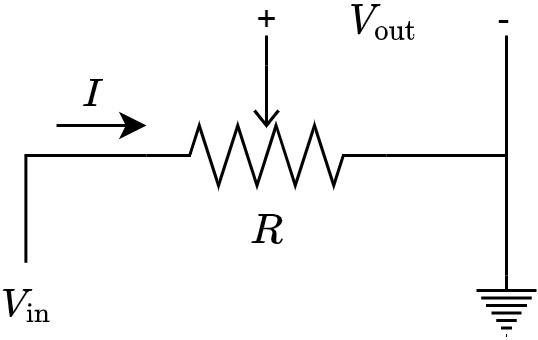
\includegraphics[scale=.5]{figs/Circuit_divide.png}
            \caption{Potentiometer}
            \label{fig:Divide_circuit_potentiometer}
        \end{subfigure}
        \begin{subfigure}{.5\textwidth}
            \centering
            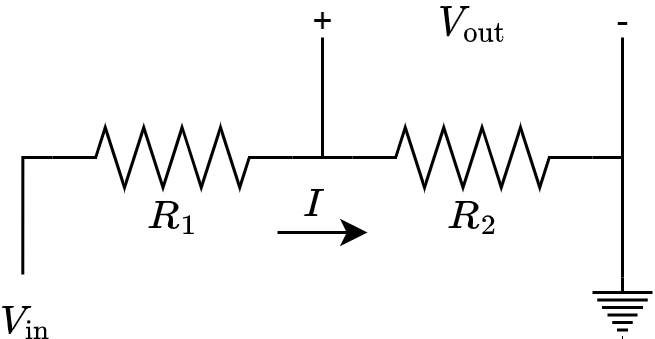
\includegraphics[scale=.5]{figs/Circuit_divide_eq.png}
            \caption{Equivalent}
            \label{fig:Divide_circuit_eq}
        \end{subfigure}
        \caption{Divide circuit}
        \label{fig:Divide_circuit}
    \end{figure}

    \section{Voltage Comparing}
    \label{ch:Voltage_comp}
    \figref{fig:Circuit_op} is the open loop operational amplifier(Op-Amp). And the relation between output voltage and input voltages is
    \begin{equation}
        V_\text{out} = A_\text{OL}\left(V_\text{p}-V_\text{n}\right)
        \label{eqn:Op_Amp}
    \end{equation}
    the $A_\text{OL}$ is the open loop gain of op-amp. In general, the gain value is huge but the power supply can't provide that high voltage. We can rewrite the \eqref{eqn:Op_Amp} become
    \begin{equation}
        V_\text{out} = \begin{cases}
            +V,\ &\text{if}\ V_\text{p}>V_\text{n}\\
            -V,\ &\text{if}\ V_\text{p}<V_\text{n}\\
            \quad 0,\ &\text{if}\ V_\text{p}=V_\text{n}
        \end{cases}
        \label{eqn:Op_comp}
    \end{equation}
    \begin{figure}[H]
        \centering
        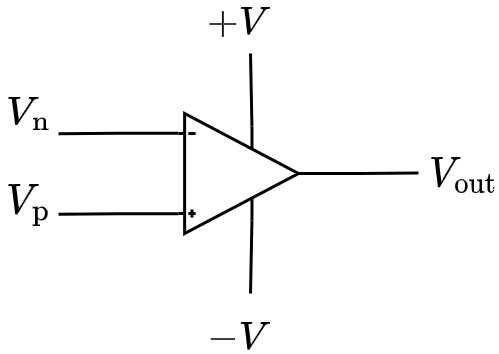
\includegraphics[scale=.5]{figs/Circuit_op.png}
        \caption{Operational amplifier}
        \label{fig:Circuit_op}
    \end{figure}

    %%% ==================== Build up NN ====================
    \chapter{Build Up Neural Network}
    \section{Introduction}
    The target of the neural network is to function like an XOR gate. So we define the neural network like \figref{fig:NN_architecture}. For the input layer, it will input True(+5V) or False(-5V). After the input layer, the signal will fully connect to the hidden layer. Each hidden node will sum up two signals after weighting. Then go through the activation function and output to the output layer. There has only one node in the output layer. Same as the hidden layer, the node in the output layer will sum up two signals after weighting and pass through the activation function. After the activation function will output the result(True or False) of the neural network.
    \begin{figure}[H]
        \centering
        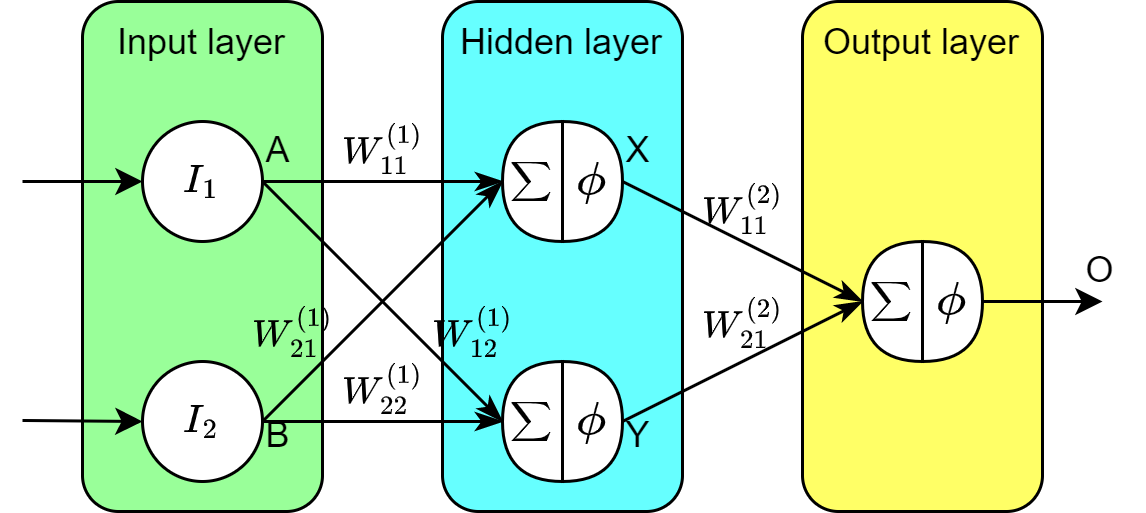
\includegraphics[scale=.3]{figs/NN.png}
        \caption{Neural network architecture}
        \label{fig:NN_architecture}
    \end{figure}

    The weighting method is using a potentiometer to divide the voltage in \chref{ch:Voltage_div}. So the weight value will between 0 and 1. And the summation method is summed up by circuit summing. From the result of \chref{ch:Voltage_sum}, the circuit summation actually is finding the average over all the input. And the activation function is using Op-Amp comparator in \chref{ch:Voltage_comp}. For \figref{fig:Op_Amp}, the comparator will compare the input and the reference voltage. If the voltage is bigger then the reference voltage, then will output the positive supply. Otherwise, will output the negative supply.
    \begin{figure}[H]
        \centering
        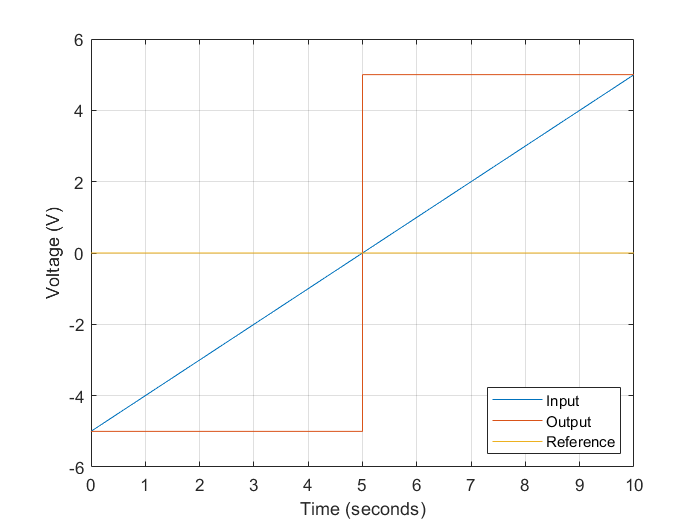
\includegraphics[scale=.6]{figs/OpAmp.png}
        \caption{Op-Amp comparator activation function}
        \label{fig:Op_Amp}
    \end{figure}

    For the beginning to build up the neural network, we need to build up the power system. The power system is like \figref{fig:Power_onboard}. There have two different voltage for the electronic components. One is $+5V$ comes from 7805 regulator for positive power supply. Another is $-5V$ comes from 7905 regulator for negative power supply. This two power will use at create the signals and amplifier's power.
    \begin{figure}[H]
        \centering
        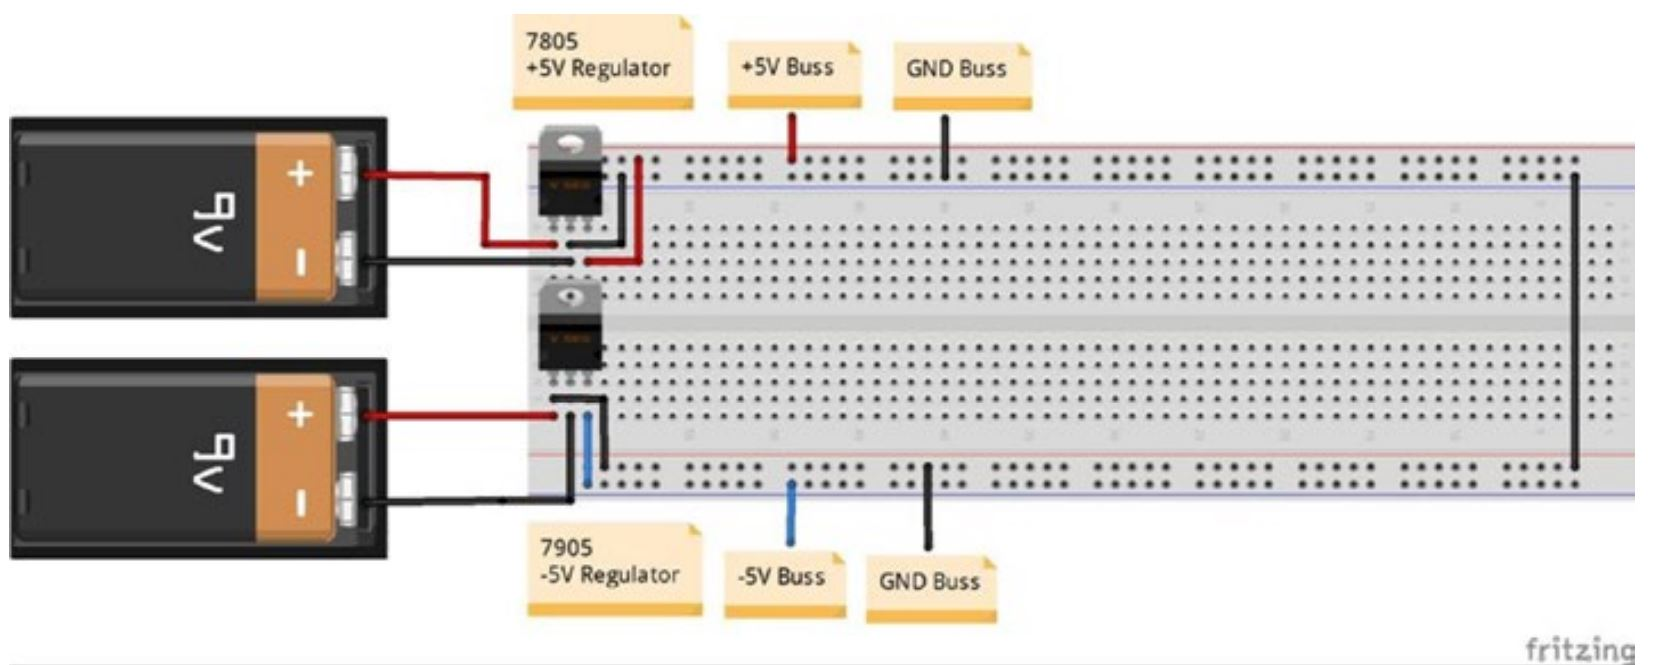
\includegraphics[scale=.4]{figs/Power_onboard.JPG}
        \caption{Protoboard power system}
        \label{fig:Power_onboard}
    \end{figure}

    \section{Input layer}
    The input layer node is present by \figref{fig:Input_layer}. The True and False signal is controlled by the SPDT switch. If the switch connects to the positive power supply, the input layer will output a True signal. Otherwise, if the switch connects to the negative power supply, the input layer will output a False signal. And we can see that there has a branch after the SPDT switch. We will connect a LED to display the state of input signal. If the LED is on, the output is True. Otherwise, the output will be False.
    \begin{figure}[H]
        \centering
        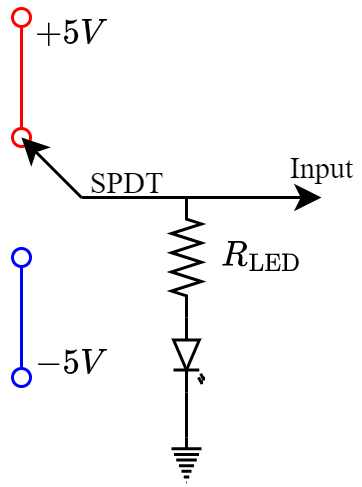
\includegraphics[scale=.7]{figs/Input_layer.png}
        \caption{Input node circuit}
        \label{fig:Input_layer}
    \end{figure}

    After adding the input layer on the protoboard will be like \figref{fig:Input_layer_onboard}.
    \begin{figure}[H]
        \centering
        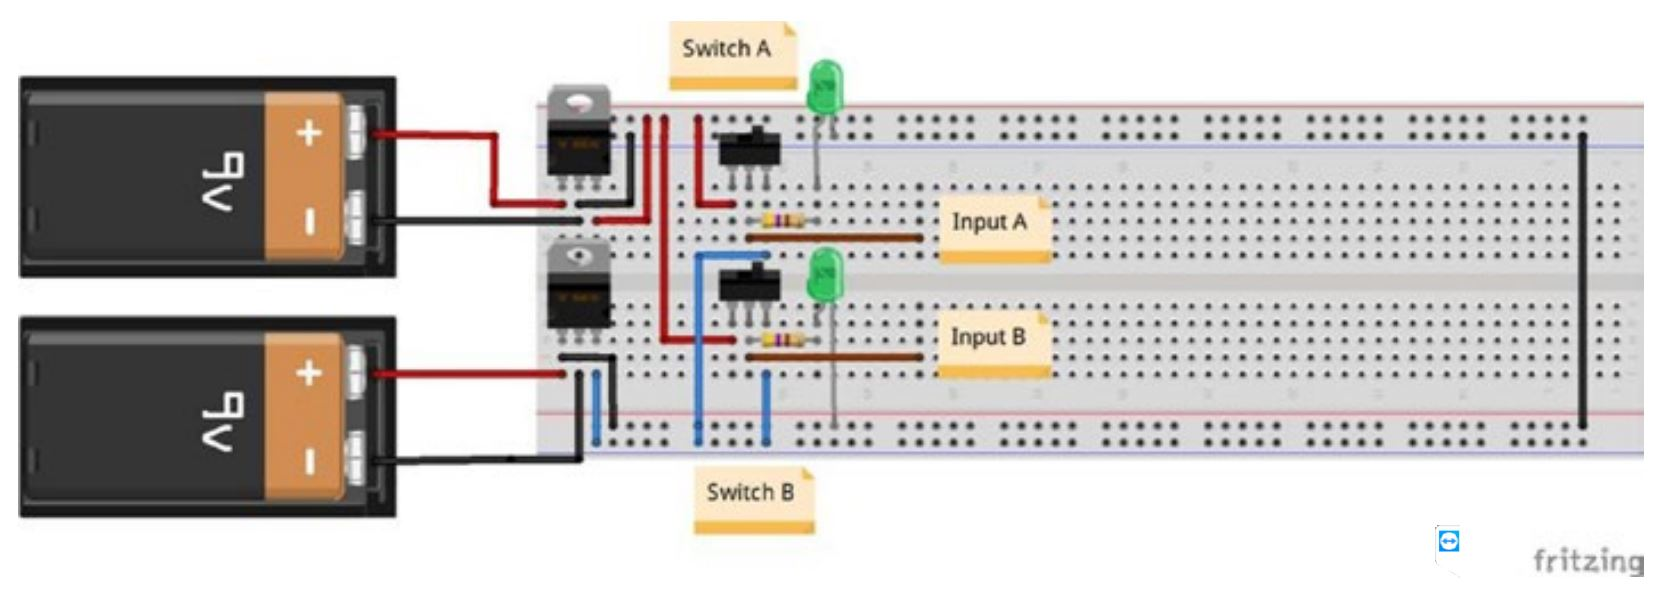
\includegraphics[scale=.4]{figs/Input_layer_onboard.JPG}
        \caption{Input layer on the protoboard}
        \label{fig:Input_layer_onboard}
    \end{figure}

    \section{Hidden layer}
    The hidden layer node is present by \figref{fig:Hidden_layer_first} and \figref{fig:Hidden_layer_secend}. For the first node in hidden layer will connect to two signal from input layer and a bias signal. And the secend node will connect to two signals from input layer. First, those signals will pass through a potentiometer to divide voltage. Next, connect two signals to two 100K$\Omega$ resistor and connect it together to get the average signals. Last after sum up, we will connect to the comparator as activation function then output.
    \begin{figure}[H]
        \centering
        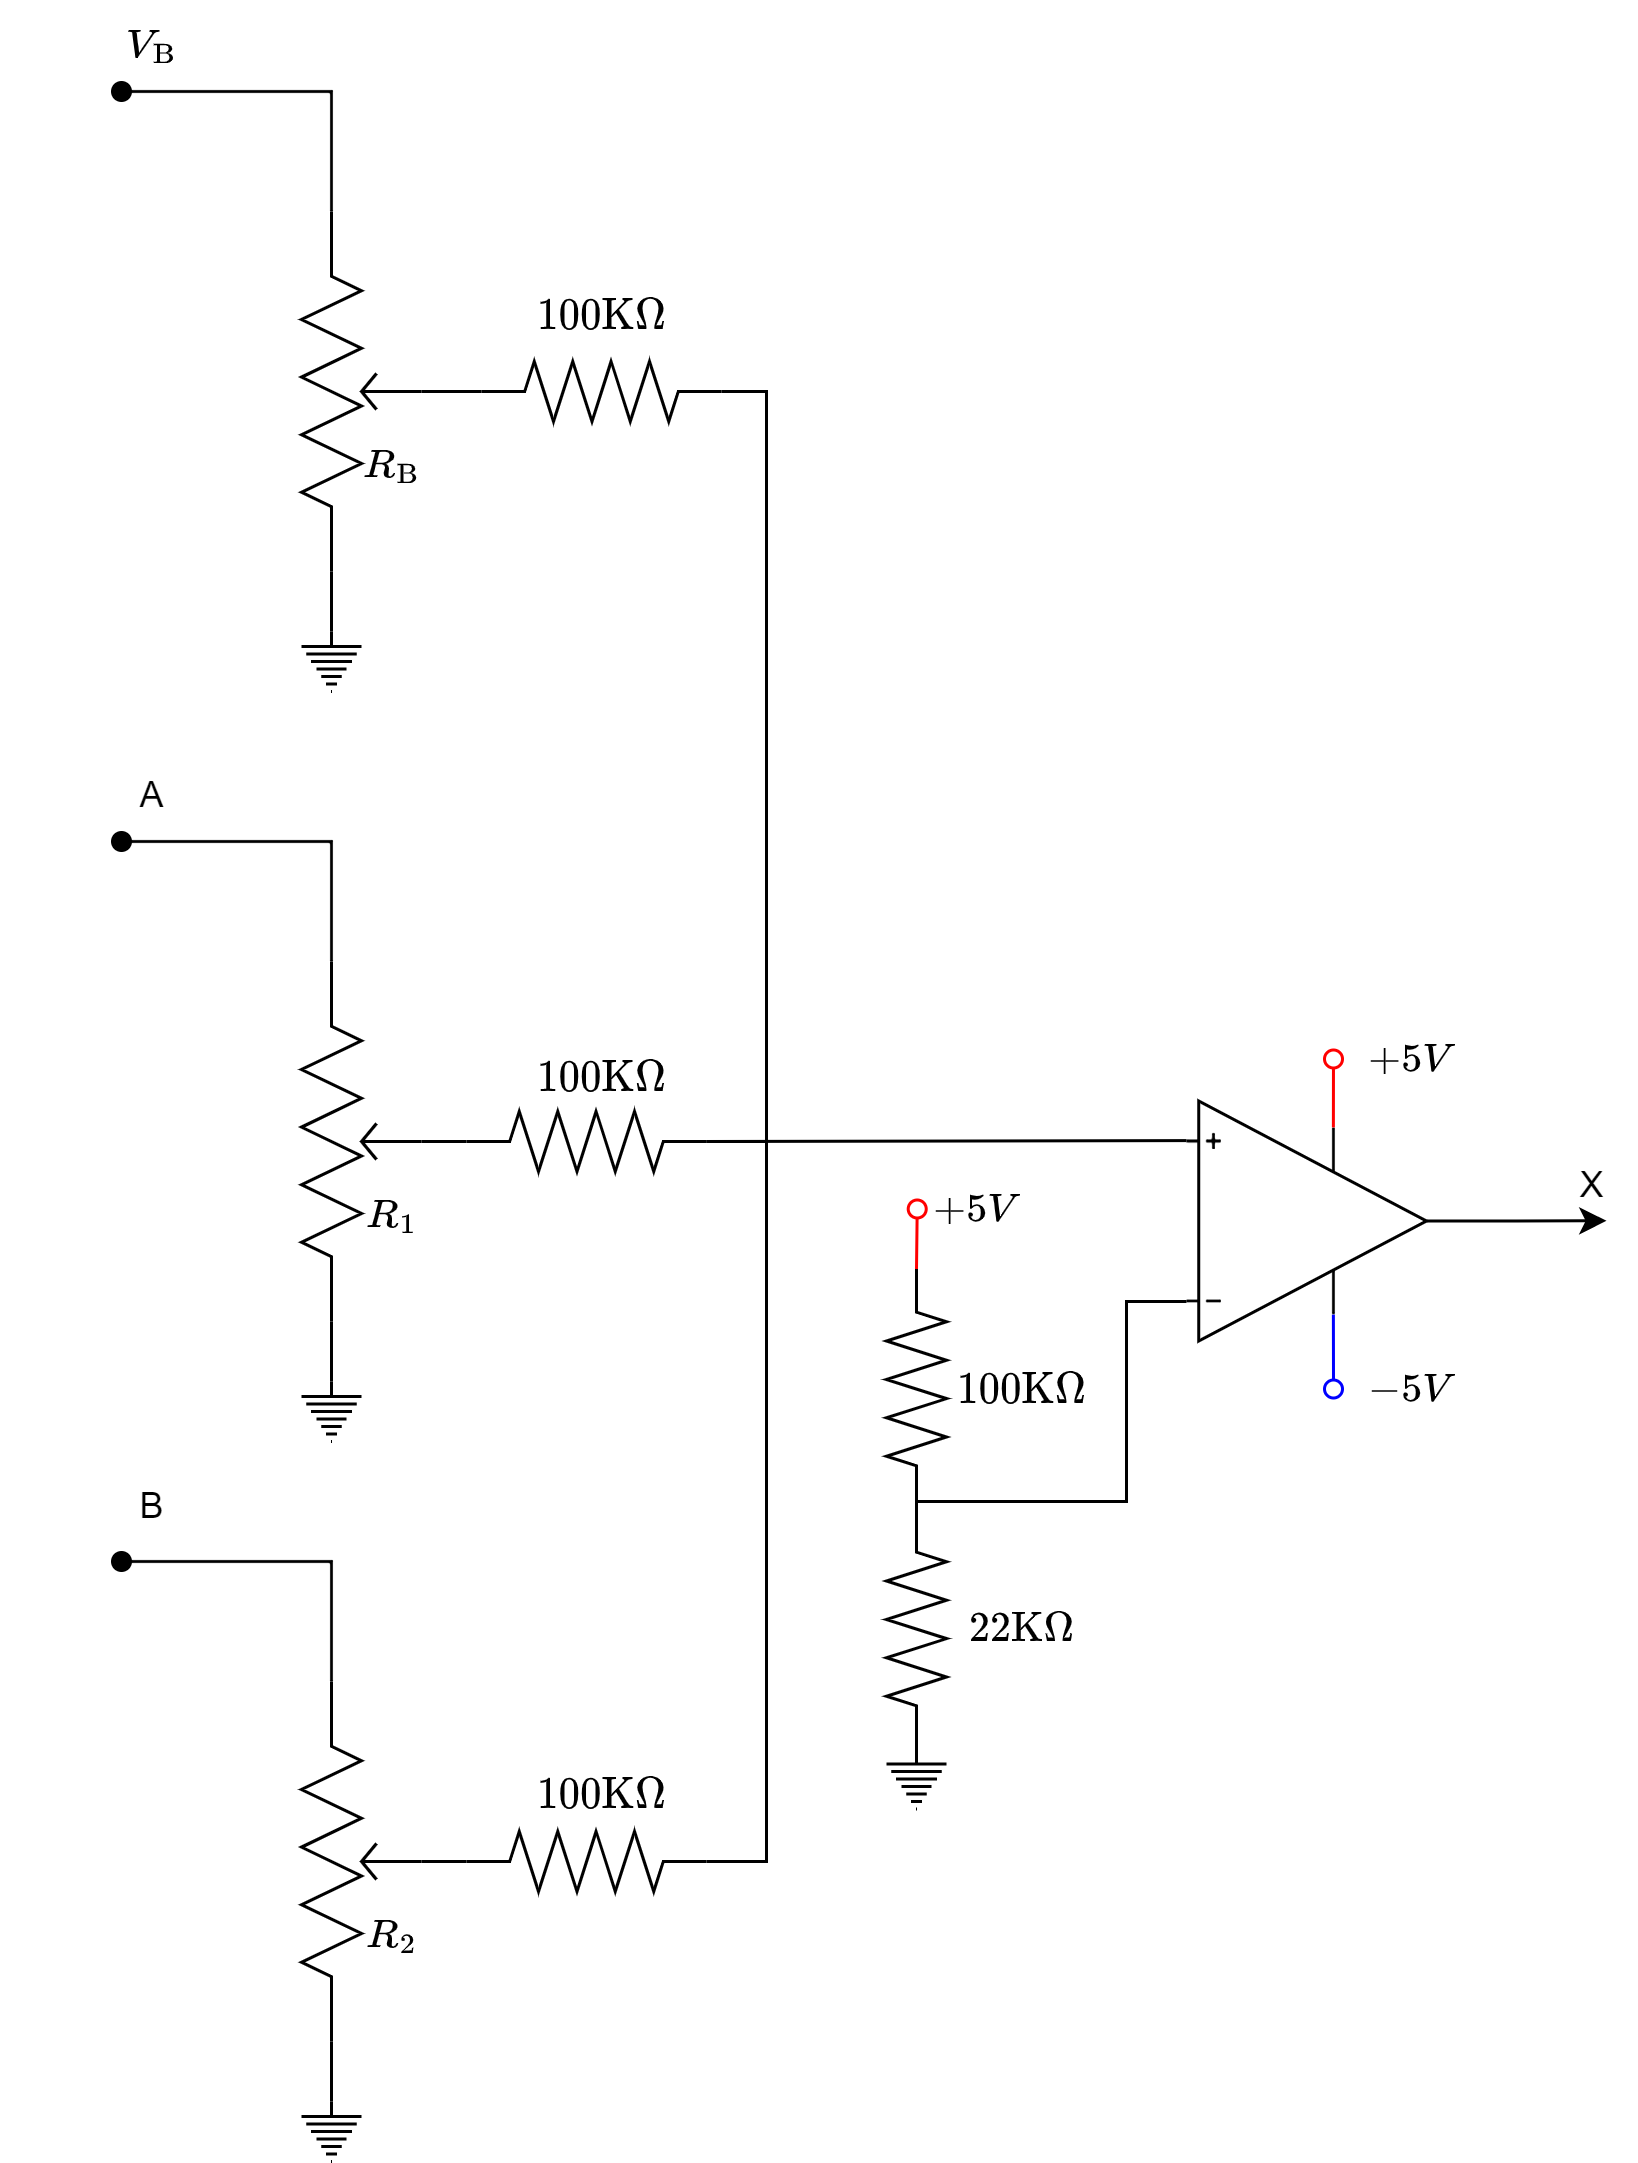
\includegraphics[scale=.2]{figs/Hidden_layer_first.png}
        \caption{First hidden node circuit}
        \label{fig:Hidden_layer_first}
    \end{figure}
    \begin{figure}[H]
        \centering
        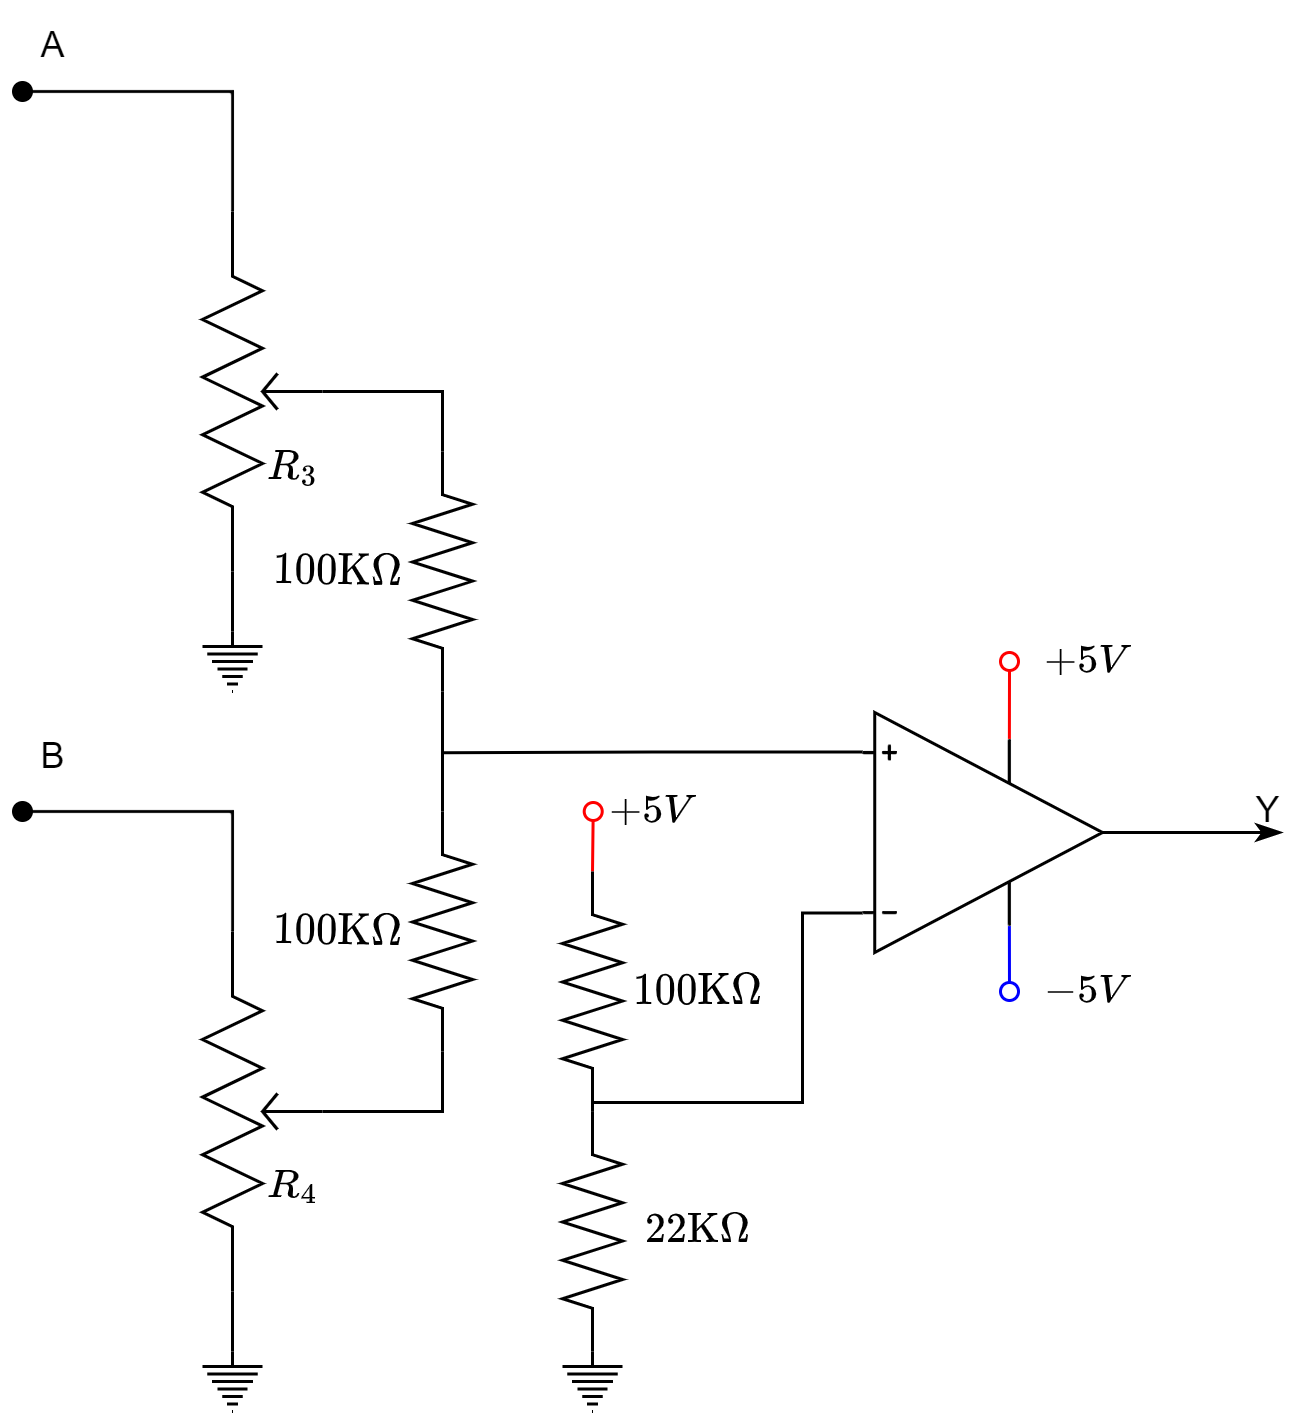
\includegraphics[scale=.2]{figs/Hidden_layer_secend.png}
        \caption{Secend hidden node circuit}
        \label{fig:Hidden_layer_secend}
    \end{figure}

    After adding the hidden layer on the protoboard will be like \figref{fig:Hidden_layer_onboard}.
    \begin{figure}[H]
        \centering
        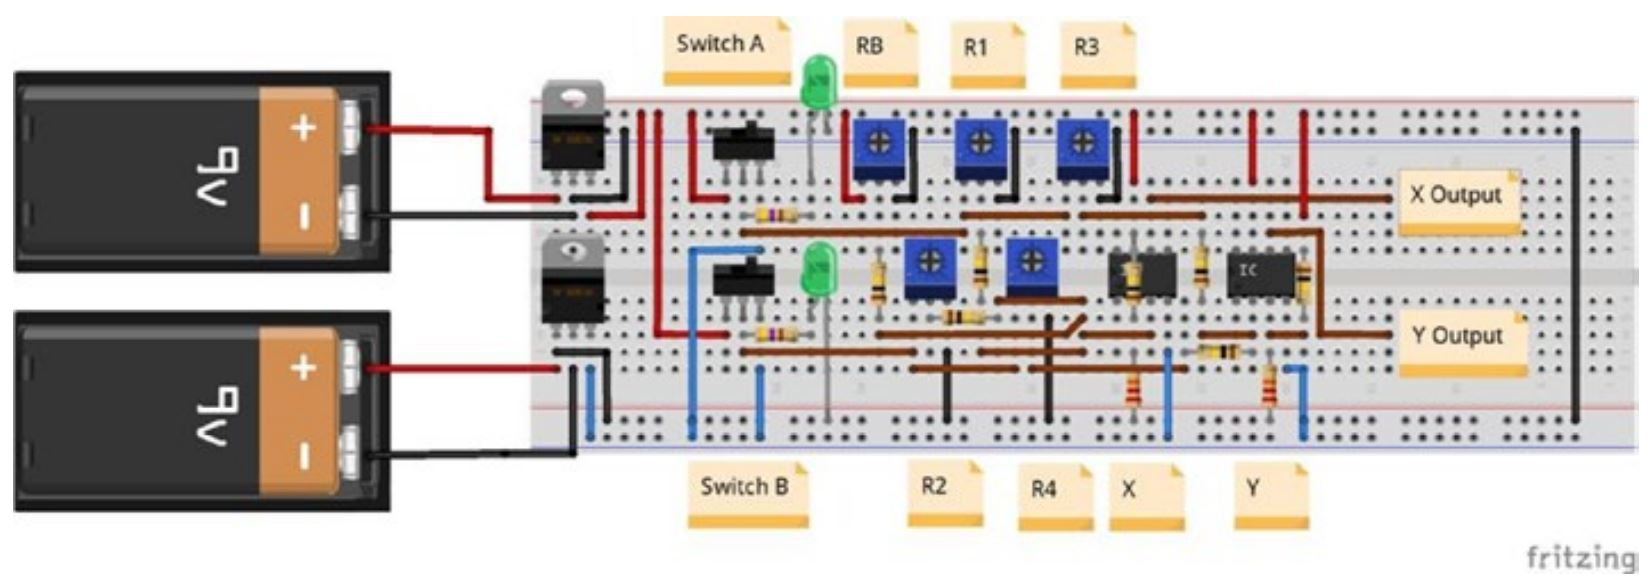
\includegraphics[scale=.4]{figs/Hidden_layer_onboard.JPG}
        \caption{Hidden layer on the protoboard}
        \label{fig:Hidden_layer_onboard}
    \end{figure}

    \section{Output layer}
    The output layer is present by \figref{fig:Output_layer}. For the output layer is similar to the hidden node. The different is the input signal $X$ and $Y$ is from the output of hidden layer. And the output will connect to a LED system to display the result.
    \begin{figure}[H]
        \centering
        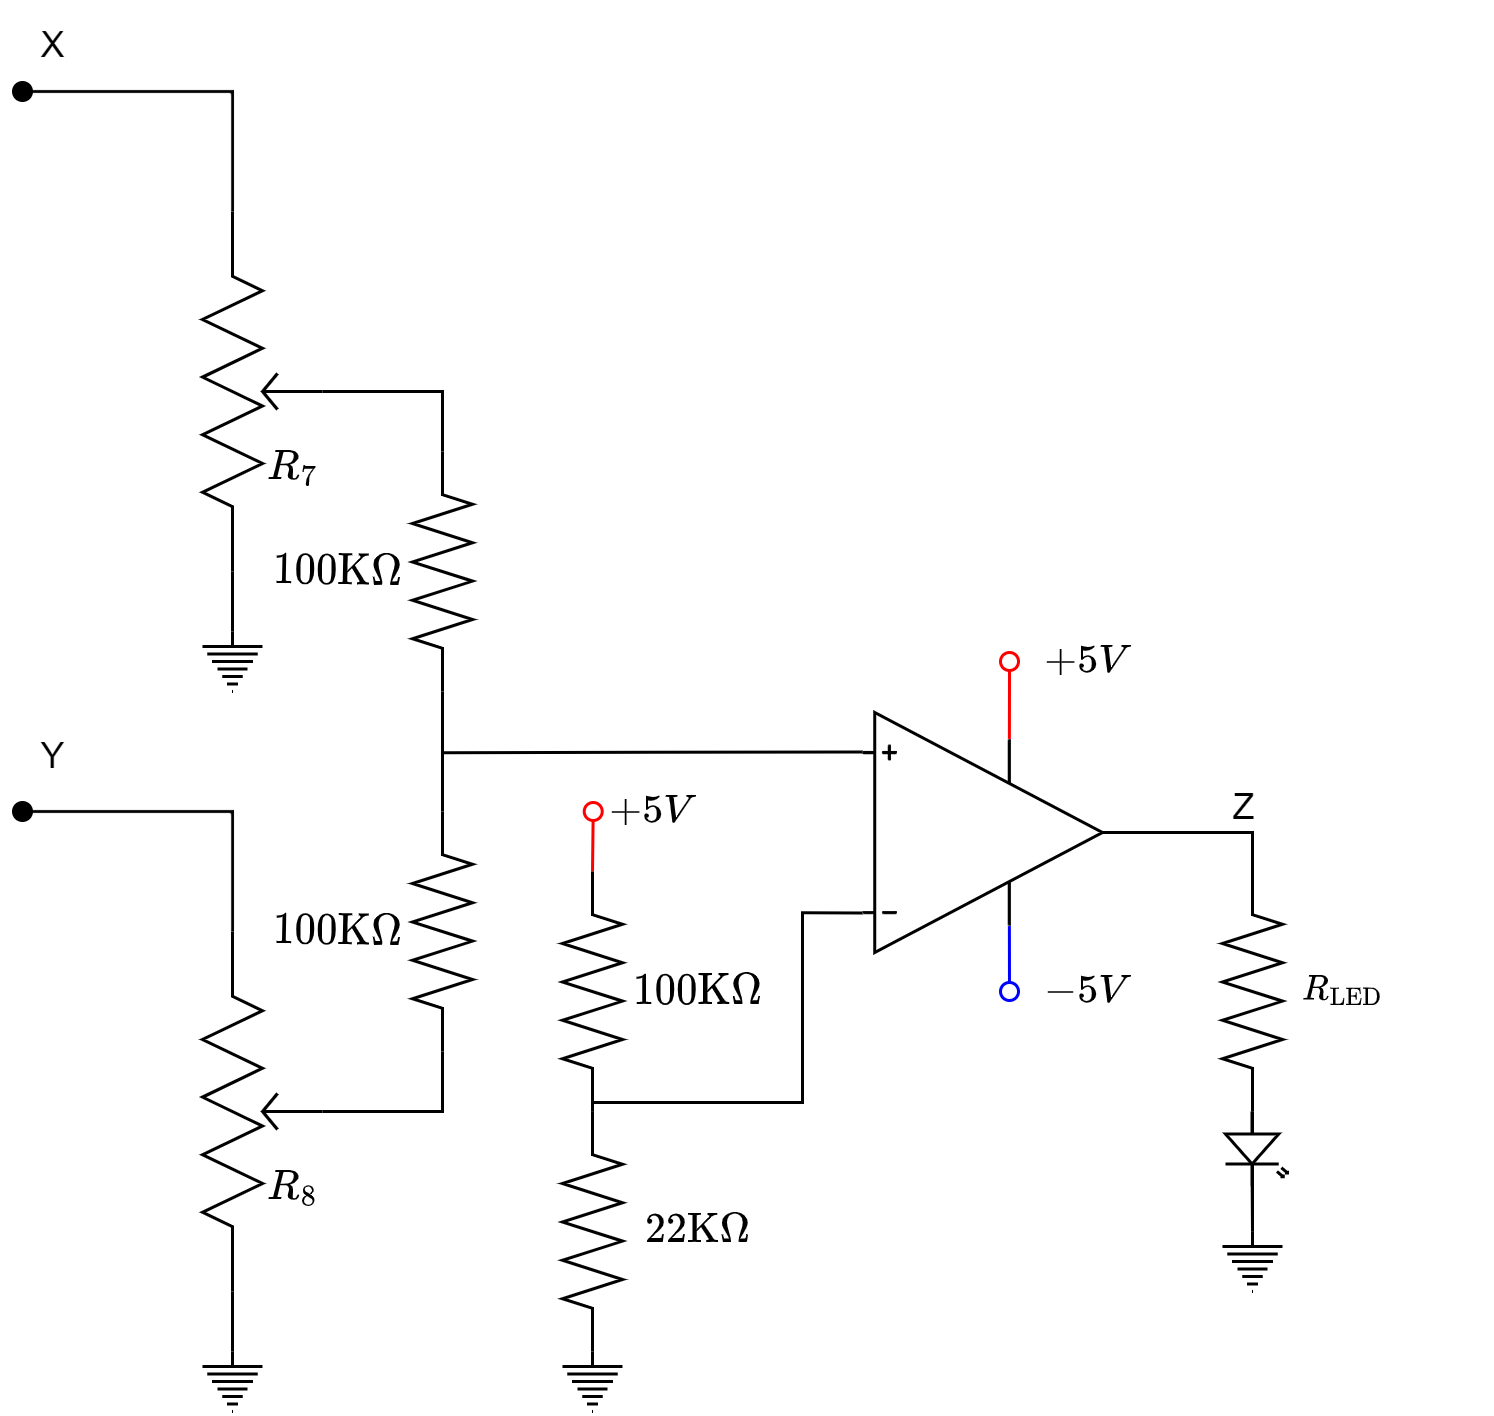
\includegraphics[scale=.2]{figs/Output_layer.png}
        \caption{Output layer circuit}
        \label{fig:Output_layer}
    \end{figure}

    After adding the output layer on the protoboard will be like \figref{fig:Output_layer_onboard}.
    \begin{figure}[H]
        \centering
        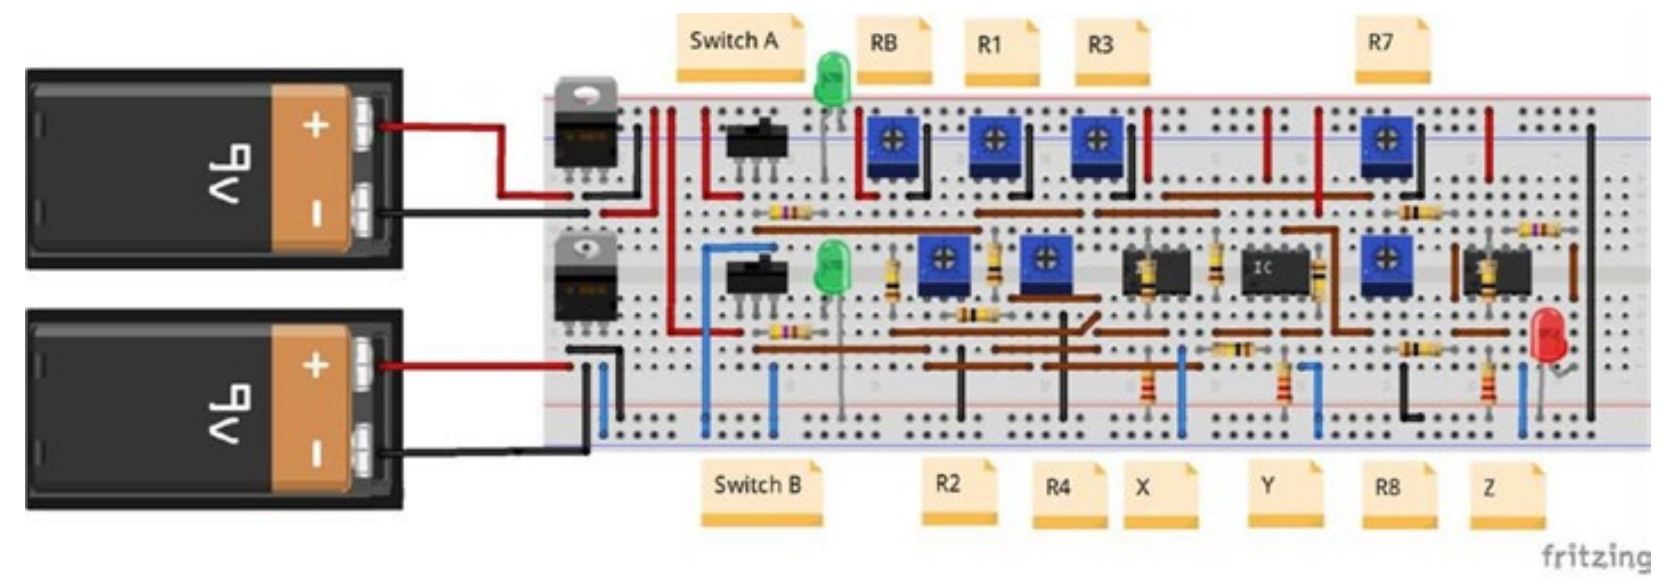
\includegraphics[scale=.4]{figs/Output_layer_onboard.JPG}
        \caption{Output layer on the protoboard}
        \label{fig:Output_layer_onboard}
    \end{figure}

    \section{Summary}
    From \figref{fig:NN_architecture} we can know that the neural network model is
    \begin{align}
        \begin{bmatrix}
            X \\ Y
        \end{bmatrix} &=
        \phi\left(\begin{bmatrix}
            W_{11}^{(1)} & W_{12}^{(1)} \\
            W_{21}^{(1)} & W_{22}^{(1)}
        \end{bmatrix}
        \begin{bmatrix}
            A \\ B
        \end{bmatrix} +
        \begin{bmatrix}
            b^{(1)}_1 \\ 0
        \end{bmatrix}\right) =
        \phi\left(v^{(1)}\right) \\
        Z &=
        \phi\left(\begin{bmatrix}
            W_{11}^{(2)} & W_{12}^{(2)}
        \end{bmatrix}
        \begin{bmatrix}
            X \\ Y
        \end{bmatrix}\right) =
        \phi\left(v^{(2)}\right)
    \end{align}
    $A$ and $B$ are the input signal, $X$ and $Y$ are the output signal of hidden layer. The weight and the bias of hidden layer is
    \begin{align}
        W^{(1)} &=
        \begin{bmatrix}
            \frac{R_1}{3\times 100} & \frac{R_2}{3\times 100} \\
            \frac{R_3}{2\times 100} & \frac{R_4}{2\times 100}
        \end{bmatrix} \\
        b^{(1)} &=
        \begin{bmatrix}
            \frac{R_\text{b}}{3\times 100} \\ 0
        \end{bmatrix}
    \end{align}
    the term of $\frac{1}{2}$ or $\frac{1}{3}$ is taking average of each node, and the term of $\frac{1}{100}$ is from voltage divide. The weight of output layer is
    \begin{equation}
        W^{(2)} =\frac{1}{2\times100}
        \begin{bmatrix}
            R_7 & R_8
        \end{bmatrix}
    \end{equation}
    For the value of resistors, $R_\text{n} \in [0, 100]$. And the activation function is
    \begin{equation}
        \phi(x) = \begin{cases}
            +5,\ &\text{if}\ x>\frac{5\times22}{122} \\
            -5,\ &\text{if}\ x<\frac{5\times22}{122} \\
            \ \ \ 0,\ &\text{if}\ x=\frac{5\times22}{122}
        \end{cases}
        \label{eqn:Comparator}
    \end{equation}


    %%% ==================== Training NN ====================
    \chapter{Training Neural Network}
    \section{Weight Tuning}
    \subsection{Back prapagation}
    For easier to analyse the neural network. We use the hyperbolic tangent function to approximate the comparator. The approximate function of \eqref{eqn:Comparator} is
    \begin{equation}
        \bar{\phi}(x) = 5\tanh\left(10\left(x-\frac{5\times22}{122}\right)\right)
        \label{eqn:Approx_comp}
    \end{equation}
    The derivative of $\bar{\phi}$ is
    \begin{equation}
        \bar{\phi}^\prime(x) = 50\left(1-\tanh^2\left(10\left(x-\frac{5\times22}{122}\right)\right)\right)
        \label{eqn:Approx_comp_derivative}
    \end{equation}
    After that we can rewrite the neural network model become
    \begin{align}
        y^{(1)} &=
        \bar{\phi}\left(W^{(1)}x+b^{(1)}\right) =
        \bar{\phi}\left(v^{(1)}\right) \\
        y^{(2)} &=
        \bar{\phi}\left(W^{(2)}y^{(1)}\right) =
        \bar{\phi}\left(v^{(2)}\right)
    \end{align}
    where $x$ is the input of neural network, $y^{(1)}$ is the output of hidden layer, and $y^{(2)}$ is the output of neural network.


    Define the loss function is square function
    \begin{equation}
        J = \frac{1}{2}(d-y^{(2)})^2 = \frac{1}{2}e^2
    \end{equation}
    $d$ is the currect value in the dataset. For the output layer,
    \begin{align}
        \frac{\partial J}{\partial W^{(2)}}
        &= \frac{\partial J}{\partial e}\frac{\partial e}{\partial y^{(2)}}\frac{\partial y^{(2)}}{\partial v^{(2)}}\frac{\partial v^{(2)}}{\partial W^{(2)}} \nonumber \\
        &= e(-1)\bar{\phi}^\prime(v^{(2)})y^{(1)^T} \nonumber \\
        &= -e\bar{\phi}^\prime(v^{(2)})y^{(1)^T} \nonumber \\
        &\triangleq -\delta^{(2)}y^{(1)^T}
    \end{align}
    The update rule of output layer will be
    \begin{equation}
        W^{(2)} \leftarrow W^{(2)} + \alpha\delta^{(2)}y^{(1)^T}
    \end{equation}
    \hrule
    For the hidden layer,
    \begin{align}
        \frac{\partial J}{\partial W^{(1)}}
        &= \frac{\partial J}{\partial e}\frac{\partial e}{\partial y^{(2)}}\frac{\partial y^{(2)}}{\partial v^{(2)}}\frac{\partial v^{(2)}}{\partial y^{(1)}}\frac{\partial y^{(1)}}{\partial v^{(1)}}\frac{\partial v^{(1)}}{\partial W^{(1)}} \\
        &= e(-1)(\bar{\phi}^\prime(v^{(2)}))(W^{(2)})(\bar{\phi}^\prime(v^{(1)}))(x^T) \\
        &= -e\bar{\phi}^\prime(v^{(2)})W^{(2)^T}\bar{\phi}^\prime(v^{(1)})x^T
    \end{align}
    The update rule of hidden layer will be
    \begin{equation}
        W^{(1)} \leftarrow W^{(1)} + \alpha e\bar{\phi}^\prime(v^{(2)})W^{(2)^T}\bar{\phi}^\prime(v^{(1)})x^T
    \end{equation}
    \hrule

   %%% ==================== Appendix ====================
    \begin{appendices}

    \chapter{Multi-input summation circuit}
    For multi-input case of \figref{fig:Summation_circuit},
    \begin{equation}
        \sum\limits_{n=1}^N I_n = 0
    \end{equation}
    replace $I_n$ by Ohm's law.
    \begin{align}
        &\sum\limits_{n=1}^N \frac{V_\text{out}-V_n}{R_n} = 0 \nonumber \\
        \Rightarrow\ &V_\text{out}\sum\limits_{n=1}^N\frac{1}{R_n} = \sum\limits_{n=1}^N\frac{V_n}{R_n}
        \label{eqn:multi_input}
    \end{align}
    For the summation of left-hand side,
    \begin{align}
        \sum\limits_{n=1}^N\frac{1}{R_n} &= \frac{1}{R_1}+\frac{1}{R_2}+\cdots+\frac{1}{R_n} \nonumber \\
        &= \frac{R_1+R_2+\cdots+R_n}{R_1R_2\cdots R_n} = \frac{\sum\limits_{n=1}^N R_n}{\prod\limits_{n=1}^N R_n}
        \label{eqn:sum_inverse}
    \end{align}
    subtitude \eqref{eqn:sum_inverse} into \eqref{eqn:multi_input}
    \begin{align}
        V_\text{out} &= \frac{\prod\limits_{n=1}^NR_n\times\sum\limits_{n=1}^N\frac{V_n}{R_n}}{\sum\limits_{n=1}^N R_n} \nonumber \\
        &= \frac{\sum\limits_{n=1}^N(\frac{1}{R_n}\prod\limits_{m=1}^NR_m)V_n}{\sum\limits_{n=1}^N R_n}
    \end{align}
    Then the result is the formula of multi-input summation.

    \end{appendices}


\end{document}